\documentclass{article}
\usepackage[utf8]{inputenc}

\title{Physics GRE}
\author{Nick Wade}
\date{March 2019}

\usepackage{lipsum}                  % imports dummy text using '\lipsum[1]'
\usepackage{geometry}                % fixes margins
\usepackage{bm}                      % bold face in math mode
\usepackage{amsmath}                 % matrix in math mode
\usepackage{indentfirst}             % Indents the first paragraph of every sections
\usepackage{hyperref}                % References to figures, eqns, and urls
\usepackage{graphicx}                % Use \includegraphics
\usepackage[font=small]{caption}     % smaller font size for captions
\usepackage{siunitx}                 % Scientific notation
\usepackage{subcaption}              % adds subfigures (two pics on one line)
\usepackage{subfiles}                % uses subfiles for sections


% example beginning and end command
\newcommand{\exbegin}{\noindent\rule{\textwidth}{1pt} \bfseries \large \vspace{0.25cm} }
\newcommand{\exend}{\vspace{0.25cm} \noindent\rule{\textwidth}{1pt} \vspace{0.25cm}}

% Line-less fraction command
\newcommand*{\bfrac}[2]{\genfrac{}{}{0pt}{}{#1}{#2}}


% sets the margins - 1.00 inch is typical for letters
\geometry{top = 1.00in,
	   bottom = 1.00in,
        inner = 1.00in,
        outer = 1.00in,
   headheight = 5ex,
      headsep = 5ex}

%% Helvetica Font
%\usepackage[scaled]{helvet}
%\renewcommand\familydefault{\sfdefault} 
%\usepackage[T1]{fontenc}











% ----------------------------------------------------------------%
% ----------------------- BEGIN DOCUMENT -------------------------%
% ----------------------------------------------------------------%
\begin{document}



% ----------------------------------------------------------------%
% ------------------------- TITLE PAGE ---------------------------%
% ----------------------------------------------------------------%
\subfile{Introduction/titlepage}
\newpage



% ----------------------------------------------------------------%
% ---------------------- TABLE OF CONTENTS -----------------------%
% ----------------------------------------------------------------%
\tableofcontents
\newpage



% ----------------------------------------------------------------%
% ------------------------ INTRODUCTION --------------------------%
% ----------------------------------------------------------------%
\section{Introduction}
\subfile{Introduction/introduction}
\newpage



% --------------------------------------------------------------------------%
% ------------------------- CLASSICAL MECHANICS ----------------------------%
% --------------------------------------------------------------------------%
\section{Classical Mechanics}


% -------------------------- SUB: INTRODUCTION -----------------------------%
\subsection{Introduction}
\subfile{Classical_Mechanics/2.1-intro/cm-intro}


% ------------------- SUB: LAWS OF MOTION AND MOMENTUM ---------------------%
\subsection{Newton's 3 Laws and the Conservation of Momentum}
\subfile{Classical_Mechanics/2.2-Newton/three-laws}


% -------------------------- SUB: PROJECTILES ------------------------------%
\subsection{Projectiles}
\subfile{Classical_Mechanics/2.3-projectiles/projectile}


% --------------------- SUB: CONSERVATION OF MOMENTUM ----------------------%
\subsection{Principle of Conservation of Momentum}
\subfile{Classical_Mechanics/2.4-momentum/momentum-conservation}


% -------------------------- SUB: CENTER OF MASS ---------------------------%
\subsection{Center of Mass}
\subfile{Classical_Mechanics/2.5-center-of-mass/center-of-mass}


% -------------------------- SUB: ANGULAR MOMENTUM --------------------------%
\subsection{Angular Momentum}
\subfile{Classical_Mechanics/2.6-angular-momentum/angular-momentum}


% ------------------------ SUB: WORK ENERGY THEOREM -------------------------%
\subsection{Work-Energy Theorem}
\subfile{Classical_Mechanics/2.7-we-theorem/work-energy}


% ------------------------- SUB: POTENTIAL ENERGY ---------------------------%
\subsection{Potential Energy}
\subfile{Classical_Mechanics/2.8-potential-energy/p-energy}


% --------------------------- SUB: CENTRAL FORCES -----------------------------%
\subsection{Central Forces}
\subfile{Classical_Mechanics/2.9-central-forces/central-forces}


% ------------ SUB: HOOKES LAW, SIMPLE HARMONIC MOTION AND ENERGY --------------%
\subsection{Hooke's Law, Simple Harmonic Motion, and Energy}
\subfile{Classical_Mechanics/2.10-SHO/simple-harmonic-motion}


% -------------------- SUB: TWO-DIMENSIONAL OSCILLATORS ------------------------%
\subsection{Two-Dimensional Oscillators}
\subfile{Classical_Mechanics/2.11-2d-osc/two-d-osc}


% ------------------------- SUB: DAMPED OSCILLATIONS ---------------------------%
\subsection{Damped Oscillators}
\subfile{Classical_Mechanics/2.12-damp-osc/damped-oscillators}


% ----------------------------- SUB: RESONANCE ---------------------------------%
\subsection{Resonance}
\subfile{Classical_Mechanics/2.13-resonance/resonance}


% ------------------------ SUB: LAGRANGE'S EQUATION ----------------------------%
\subsection{Lagrange's Equation}
\subfile{Classical_Mechanics/2.14-lagrange/lagrange-equation}


% ----------------------- SUB: TWO-BODY CENTRAL FORCES -------------------------%
\subsection{Two-Body Central Forces}
\subfile{Classical_Mechanics/2.15-two-central-forces/2-body-central-forces}


% --------------------------- SUB: ORBITAL EQUATIONS -----------------------------%
\subsection{Orbital Equations}
\subfile{Classical_Mechanics/2.16-orbital-eqns/orbital-equations}


% --------------------------- SUB: KEPLERIAN ORBITS -----------------------------%
\subsection{Keplerian Orbits}
The Kepler problem is to find the possible orbits of an object subject to an inverse-square force.








\newpage
% --------------------------------------------------------------------------%
% ---------------------------- ELECTROMAGNETISM ----------------------------%
% --------------------------------------------------------------------------%
\section{Electromagnetism}
\subfile{Electromagnetism/2.1-intro/em-intro}





\newpage
% --------------------------------------------------------------------------%
% ----------------------------- MISC. TOPICS -------------------------------%
% --------------------------------------------------------------------------%
\section{Miscellaneous Topics}


% --------------------------- SUB: POLAR COORDINATES -----------------------------%
\subsection{Polar Coordinates}

As derived from a Cartesian plane, the conversion equations are known to be:

\begin{table}[h]
    \centering
    \begin{tabular}{c}
        $x = rcos\phi$ \\
        $y = rsin\phi$ \\
        $r = \sqrt{x^2 + y^2}$ \\
        $\phi = arctan(y/x)$
    \end{tabular}
\end{table}

Solving problems using polar coordinates sometimes makes or break a 2 minute question for you on the GRE. Often times, these are used to solve for rotational motion problems (pendulum or professor in a half-pipe). Being able to quickly derive the derivatives of spherical coordinates is extremely important if you want to solve these problems quickly. 

\begin{figure}[h]
    \centering
    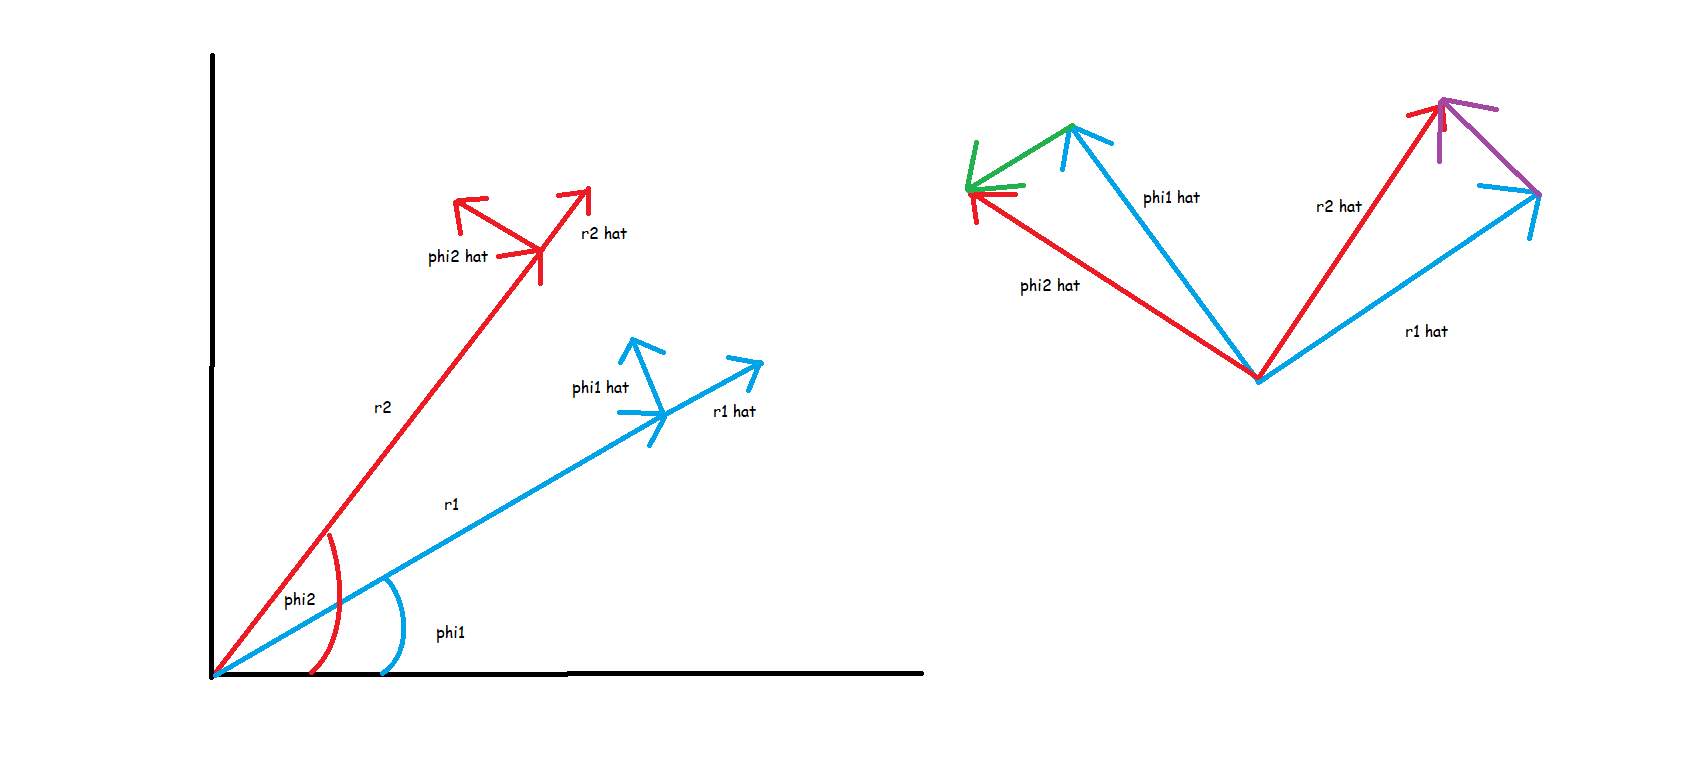
\includegraphics[width=13.0cm]{Misc/3.1/spherical-derive.png}
    \caption{Vector $\vec{r}_1$ is blue and $\vec{r}_2$ is red. To the right, the differences in the unit vectors are shown as a small amount of time is lapsed. The green and purple lines shown $\Delta \hat \phi$ and $\Delta \hat r$, respectively. Notice the directions of these resultant vectors.}
    \label{fig:spherical-coord-deriv}
\end{figure}

Both $\hat \dot r$ and $\hat \dot \phi$ have a similar derivation. Consider a situation such as the one in figure \ref{fig:spherical-coord-deriv}. $|r_1|$ and $|r_2|$ are equal. In this scenario, $\phi_1$ is increased by some amount $\Delta \phi$, that is $\phi_2 = \phi_1 + \Delta \phi$. This changes $\hat \dot r$ by a small amount over a time interval $\Delta t$. From the above picture, we can deduce,

\begin{equation}
    \label{eqn:polar-coord-deriv1}
    \Delta \hat r \approx \Delta \phi \hat \phi \approx \dot \phi \Delta t \hat \phi
\end{equation}

\noindent provided $\Delta t$ is small. Dividing both sides of equation \ref{eqn:polar-coord-deriv1} by $\Delta t$ and taking the limit as $\Delta t \rightarrow 0$,

\begin{equation}
    \label{eqn:polar-coord-deriv2}
    \frac{d \hat r}{dt} = \dot \hat r = \dot \phi \hat \phi.
\end{equation}

Looking at equation \ref{eqn:polar-coord-deriv2}, can conclude that $\Delta \hat r$ is directly proportional to $\Delta \hat \phi$. Similarly, we can deduce, 

\begin{equation}
    \label{eqn:polar-coord-deriv3}
    \frac{d \hat \phi}{dt} = - \dot \phi \hat r.
\end{equation}

Finally, we can arrive at a similar situation of deriving the position function to find the acceleration function. Starting with $\vec{r}(t) = r \hat{r}$ and utilizing the product rule for differentiation,

\begin{equation}
    \label{eqn:polar-coord-deriv4}
    \frac{d\vec{r}}{dt} = \frac{d}{dt}[r \hat r] \rightarrow \dot r = \frac{dr}{dt} \hat r + \frac{d \hat r}{dt} = \dot r \hat r + \dot \phi r \hat \phi.
\end{equation}

\noindent Differentiating equation \ref{eqn:polar-coord-deriv4} again,

\begin{equation}
    \label{eqn:polar-coord-deriv5}
    \vec{a} = \frac{d}{dt}[\dot r \hat r] + \frac{d}{dt}[r \dot \phi \hat \phi] \rightarrow (\ddot r - r \dot \phi^2) \hat r + (2\dot r \dot \phi + r \ddot \phi) \hat \phi.
\end{equation}

The best way to understand equation \ref{eqn:polar-coord-deriv5} is the think of a stone tied to the end of a rope and swung in a circle, that is have $\dot r = 0$. Solving this, you will find terms such as centripetal acceleration, $r \omega^2$, where $\omega$ is the angular velocity $\dot \phi$, and angular acceleration, $\alpha = \ddot \phi$.


% --------------------- SUB: LINEAR DIFFERENTIAL OPERATORS ------------------------%
\subsection{Linear Differential Operators}

Just to clean up the notation, as this is most appropriate for the topic of driven damped oscillators: $D = \frac{d^2}{dt^2} + 2\beta \frac{d}{dt} + \omega_o^2$. $D$ is  a {\itshape differential operator} that cleans up the equation for the solving driven damped oscillator equation, which now becomes $Dx = f$. Most importantly, $D$ is linear. This is only true if the operator is commutative and distributive - in a sense. For example,

\begin{equation*}
    D(ax_1 + bx_2) = aDx_1 + bDx_2.
\end{equation*}

\noindent Any operator that satisfied this equation is considered {\itshape linear}.

A {\bfseries homogeneous} equation is $Dx=0$ (the undriven damped oscillator). This is solved with a {\bfseries homogeneous solution}, $x_h$ in $Dx_h=0$. On the other hand, a {\bfseries inhomogenous} equation is $Dx=f$ (the driven damped oscillator). This is solved with a {\bfseries particular solution}, $x_p$ in $Dx_p=f$.




\end{document}
